\section{COMPLETUDE DOS DADOS}

\begin{figure}[htb!]
    \centering
	\captionsetup{justification=raggedright, singlelinecheck=false, width=1\textwidth}
    \caption{Gráfico de completude dos dados para o mês de MÊS para estação ESTAÇÃO.}
    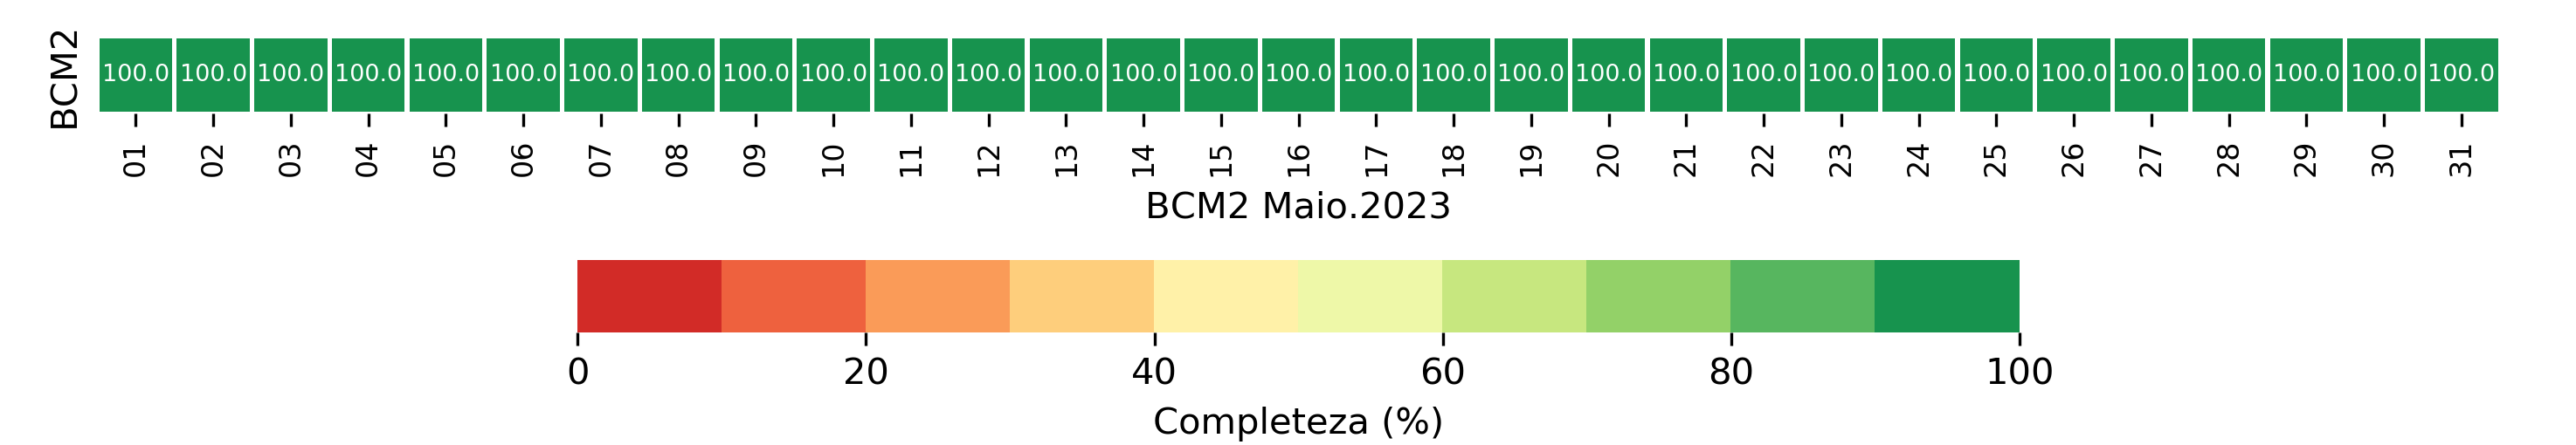
\includegraphics[width=1.0\textwidth]{./figuras/completude.png} % Substitua pelo nome da imagem e ajuste o tamanho
    \caption*{Fonte: IPT}
    \label{fig:completude}
\end{figure}

